\section{Itération~0:~(~2/20/2017~-~2/22/2017~)}
\subsection{Introduction}
\subsection{Objectif de l'itération}

Avant de commencer la première itération du Scrum, une période de temps à été
consacrée pour préparer ce qui est nécessaire au lancement du projet dans de
bonnes conditions. Cette période est souvent nommé l'itération 0 du projet.
Elle est consacrée généralement à la recherche bibliographique, aux choix
technologiques et à la mise en place de l'environnement de développement. Autre
que ces préparatifs, c'est dans cette itération que nous définissons le Backlog
de la plateforme, ainsi que le nombre d'itérations nécessaires et la durée de
l'itération. Il s'agit aussi d'une période de formation pour les membres de
l'équipe sur tous les environnements et les technologie à utiliser au cours du
montage du produit.

\begin{figure}[htbp]
  \centering
  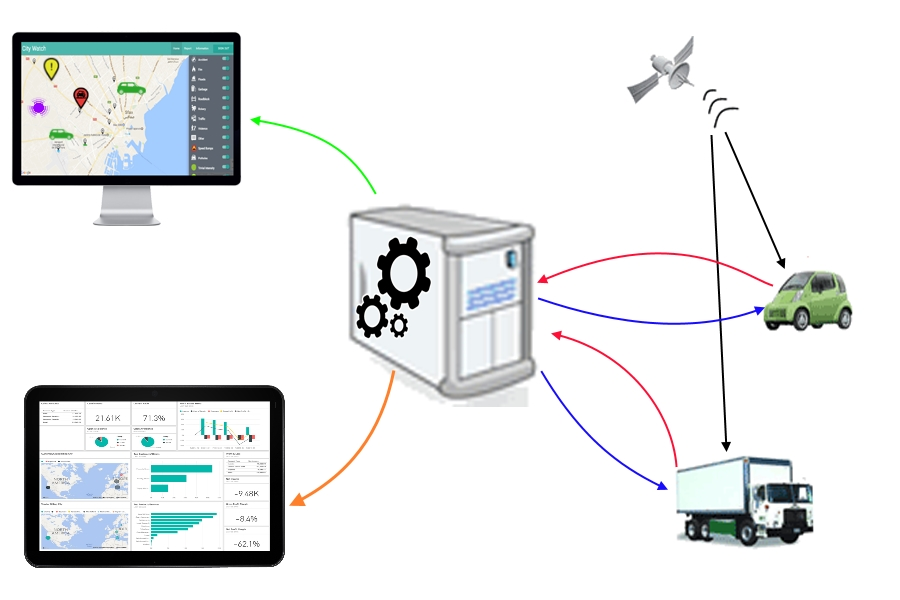
\includegraphics[width=0.8\textwidth]{citywatch-architecture}
  \caption[Flux des information Géographiques en CityWatch]
  {Flux des informations Géographiques dans le système de localisation}
  \label{fig:citywatch-architecture}
\end{figure}

\subsection{Backlog générale}

La première étape de la méthode Scrum consiste à préparer un carnet du produit
(Product Backlog) qui présente la liste des tâches à effectuer durant le
développement du projet qui sera répartie en des itérations. Le rôle du
Product Owner est important dans cette phase de développement parce qu'il devra
faire l'exercice de prioriser ses demandes selon des critères respectant la
mission et les objectifs de son produit. En précisant la valeur de priorité, il
estime l'impact et le retour sur investissement qu'aura chacun des items dans
le carnet du produit. Il y a donc effectivement eu un gros travail d'échanges
et discussions avec le client pour comprendre tout le cahier des charge
initial, C'est comme ça que le Backlog a été défini.

Les valeurs d'affaires sont définies comme suit :
\begin{description}[align=right,labelwidth=1cm]
    \item [1] Définie une haute priorité, affectée pour les spécifications
        importantes, exigées pour le produit.
    \item [2] Définie une priorité importante mais pas exigée.
    \item [3] Définie une priorité moyenne ou parfois faible.
\end{description}

La figure~\ref{fig:product-backlog} présente une version simplifiée du Product
Backlog complète des 3 premières itérations. Nous représentons notre
participation par les cercles du texte souligné.

\usetikzlibrary{mindmap,shadows}
\newcommand*{\info}[4][16.3]{%
  \node [ annotation, #3, scale=0.65, text width = #1em,
          inner sep = 2mm ] at (#2) {%
  \list{$\bullet$}{\topsep=0pt\itemsep=0pt\parsep=0pt
    \parskip=0pt\labelwidth=8pt\leftmargin=8pt
    \itemindent=0pt\labelsep=2pt}%
    #4
  \endlist
  };
}
\begin{figure}[htbp]
%\usepackage{dtklogos}
\hspace{-9ex}
\begin{tikzpicture}[every annotation/.style={draw, fill=white, font=\Large}]
    \renewcommand{\href}[2]{#2}

    \path[mindmap,
          concept color=black!40,
          text=white,
          every node/.style={
              concept,
              circular drop shadow,
              execute at begin node=\hskip0pt,
          },
          %grow cyclic,
          root/.style={
              concept color=black!40,
              fill=white, line width=1ex, text=black,
              font=\footnotesize\bfseries,
              text width=7em},
          level 1 concept/.append style={
              font=\normalsize\bfseries,
              sibling angle=50,
              text width=7.7em,
              level distance=12.5em,
              inner sep=0pt},
          level 2 concept/.append style={
              font=\footnotesize\bfseries,
              level distance=8em},
          ours/.append style = {
              line width=0.5ex,
              concept color = black,
          }
    ]

    node[root] {Platforme CityWatch} [clockwise from=0]

    child[concept color=blue!70] {
        node {\ul{Gestions des Rapports}} [clockwise from=50]
        child { node { \ul{Consultation} } }
        child { node { \ul{D\'eclaration} } }
    }
    child[concept color=green!40!black] {
        node[concept] {\ul{Information Routi\`ere}} [clockwise from=30]
        child { node[concept] {\ul{Secousses}} }
        child { node[concept] {\ul{Ralentisseurs}}}
        child { node[concept] {Embouteillage}}
    }
    child[concept color=blue] {
        node[concept] {\ul{Itin\'eraire}} [clockwise from=305]
        child { node[concept] {\ul{Localisation instantan\'e}} }
        child { node[concept] {\ul{Projection du Trajectoire}} }
        child { node[concept] {\ul{Historie des Trajectoires}} }
    }
    child[concept color=red!60!black] {
        node[concept] {Assistance} [clockwise from=235]
        child { node[concept] {Alerte des secousses} }
        child { node[concept] {Alerte des ralentisseurs} }
    }
    child[concept color=orange] {
        node[concept] {\ul{Tableau de Bord}} [counterclockwise from=100]
        child { node[concept] {\ul{Carte en Temps R\'eel}}}
        child { node[concept] {\ul{Authentification}} }
        child { node[concept] {\ul{Filtrages}} }
    }
    child[concept color=yellow!60!black] {
        node[concept] (Blogs) {\ul{Analyse et Visualisation}} [clockwise from=135]
        child { node[concept] {Visualisation des données}}
        child { node[concept] {\ul{Tableau du bord interactive}}}
    }
    child[concept color=red] {
        node[concept] {Information Réseau} [clockwise from=110]
        child { node[concept] {Signal Réseau} }
        child { node[concept] {Génération Réseau} }
        child { node[concept] {Opérateur Réseau} }
    };
\end{tikzpicture}
\caption{Objective du produit}
\label{fig:product-backlog}
\end{figure}


Le tableau~\ref{tab:product-backlog} représente la liste plus détaillé des cas
d'utilisations que nous allons implémentés pendant les 3 premières itérations.
Ils suivent la forme:
\begin{displayquote}
    En tant que \textbf{X}, je peux \textbf{Y} Afin d'\textbf{Z}.
\end{displayquote}
ou aussi la forme:
\begin{displayquote}
    En tant que \textbf{X}, je veux qu'il soit possible de \textbf{Y} pour
    \textbf{Z}.
\end{displayquote}

Dans notre liste des cas d'utilisation, l'acteur initiateur (\textbf{X}) est
toujours l'utilisateur.

\Needspace{5\baselineskip}
\begin{center}
    \footnotesize
    \setlength\LTleft{-20pt}
    \begin{longtable}{| l | p{3.5cm} | p{5.5cm} | p{5cm} | l |}
 \caption{Backlog du Produit}
 \label{tab:product-backlog} \\

 \hline
 \textbf{ID} & \textbf{Cas d'utilisation} & \textbf{Je veux qu'il soit possible de} & \textbf{Pour} & \textbf{Priorité} \\ \hline
 \endhead

 \hline \multicolumn{5}{|r|}{{Continué en page suivante$\dotsc$}} \\ \hline
 \endfoot

 \hline \hline
 \endlastfoot

\hline
%1 & Gestion du Trajectoire & démarrer le localisation & Avoir un feedback dans l'application et sur le site web & 1 \\ \cline{3-5}
%  &                        & arrêter le localisation & Avoir un feedback dans l'application & 1 \\ \hline
%2 & Gestion de Rapports    & choisir entre une variété de problèmes à déclarer depuis l'application & Avoir un feedback sur le site web & 1 \\ \cline{3-5}
%  &                        & choisir l'emplacement du problème à déclarer dans une carte & Avoir un feedback sur le site web & 1 \\ \cline{3-5}
%  &                        & ajouter une description ou une image au problème & Avoir un feedback sur le site web & 2 \\ \hline
%3 & Consulter la carte     & consulter la carte depuis l'application & Voir la carte dans l'application & 2 \\ \hline
%4 & Compte                 & consulter le site web sans avoir un compte & Consulter le site web avec un minimum d'informations & 1 \\ \cline{3-5}
%  &                        & créer un compte & Avoir un compte personnel & 2 \\ \hline
%5 & Groupement des rapports& voir les rapports en groupe lors d'un zoom out & Avoir une vision globale sur le nombre des rapports & 1 \\ \hline
%6 & Déclarer un rapport    & déclarer un rapport à partir du site web & Avoir accès à une page rapport comme celle de l'application & 1 \\ \hline
% \hline \ldots & \ldots & \ldots & \ldots & \ldots \\ \hline

%
1 & Gestion du Trajectoire & Activer le localisation & Enregistrer le trajectoire & 1 \\ \cline{3-5}
&                          & Consulter le dashboard  & Afficher le trajectoire instantané & 1 \\ \cline{3-5}
&                          & Filtrer le trajectoire  & Consulter l'histoire des trajectoires & 2 \\ \hline
2 & Gestion des Rapports   & Déclarer un rapport depuis le site & Avoir un rapport dans la carte & 1 \\ \cline{3-5}
&                          & Choisir un emplacement & Afficher et filtrer par catégorie & 1 \\ \cline{3-5}
&                          & Ajouter une image et commentaire & Enrichir le rapport & 1 \\ \cline{3-5}
&                          & Accéder à formulaire depuis l'application mobile & rapporter instantané et facilement & 2 \\ \cline{3-5}
&                          & Activer/Désactiver le groupement des marqueurs & Avoir une vision sur le nombre des rapports plus claire & 3 \\ \hline
3 & Tableau de bord (Dashboard) & Consulter le dashboard & Visualiser diffèrent type de données comme marqueurs et zones & 1 \\ \cline{3-5}
&                               & Manipuler la légende    & Filtrer les données affichés & 1 \\ \hline
4 & Comptes                & Créer un compte & Pouvoir enregistrer des données personnels (trajectoire) & 3 \\ \cline{3-5}
&                          & Se connecter & Accéder au données routières privées (trajectoire) & 3 \\ \cline{3-5}
&                          & Visiter le dashboard sans compte & Consulter une version minimale des fonctionnalités & 3 \\
\hline
\end{longtable}
\end{center}

\subsection{Préparation de l'environnement du travail}

\subsubsection{Environnement logiciel}

La réalisation de ce projet nécessite l'ensemble de ces logiciels et
bibliothèques:

\paragraph{Android}

On a choisi du supporter le système Android comme notre première plateforme. Ce
choix était basé sur différents aspects:
\begin{itemize}
    \item La part de marché des smartphones et tablettes Android.
    \item L'ouverture de la plateforme, et l'accessibilité aux différentes
        fonctionnalités et aux outils de développements.
    \item Android Auto, Android Wear, Android Things\ldots
\end{itemize}

Android Studio était le choix naturel pour le développement d'application
grâce au support officiel du Google et les fonctionnalités héritées de l'ide
IntelliJ IDEA de JetBrains comme un concepteur d’interface utilisateur pour
des résolutions variées simultanément, débogueur, \ldots

%\subparagraph{Android studio}
%est un environnement de développement pour développer des applications Android.
%Il est basé sur IntelliJ IDEA.\\ Android studio permet principalement d'éditer
%les fichiers Java et les fichiers de configuration d'une application Android.Il
%propose entre autres des outils pour gérer le développement d'applications
%multilingues et permet de visualiser la mise en page des écrans sur des écrans
%de résolutions variées simultanément

\paragraph{PHP}
En se basant sur les conseils du Product Owner et aux limites d'environnement
de développement dont le serveur supporte seulement PHP, on a choisi la langue
de programmation PHP\@.
Les points fort de la langue PHP:
\begin{itemize}
    \item Une langue très répondu dans le développement Web, Elle a une
        grande communauté des développeurs.
    \item Une grande liste des outils de développement incluant les
        gestionnaires des dépendances (Composer, Phar), outils des tests
        unitaires (PHPUnit), générateurs du documentation (PHPDoc, Sami),
        débogueurs (Xdebug), analyseurs du code et analyseurs statiques
        (php\_CodeSniffer, PHPLint), outils d'automatisation (Phing) and
        multiple IDEs.
    \item Multiple bibliotheques et frameworks pour différent type des projets.
\end{itemize}

Les points faibles de la langue PHP:
\begin{itemize}
    \item Gestion d'erreurs très souple par défaut même si les erreurs sont
        fatales.
    \item Manque d'un paradigme unique dans l'architecture de la langue (le
        choix du syntaxe et du noms des fonctions)
\end{itemize}

L'ide choisie pour le développement PHP est PHPStorm, un IDE multiplatforme de
JetBrains. Il regroupe sous une interface conviviale un éditeur de
texte avancé et intelligent, un interpréteur et un débogueur\ldots.
Vim a été aussi utilisé avec un ensemble des extensions pour enrichir ses
fonctionnalités.

%\paragraph{Composer}
%
%Le logiciel Composer est un gestionnaire de dépendances sous licence libre
%écrit en PHP\@. Il permet à ses utilisateurs de déclarer et d'installer les
%bibliothèques dont le projet principal a besoin.

\paragraph{Technologies du Web}

\TODO{Wht HTML5, CSS3, JS}

\subsubsection{environnements matériels}

Pour le développement de ce projet, il était demandé d'avoir :
\begin{itemize}
 \item Serveur Local pour les tests
     \begin{itemize}
         \item Windows 10
         \item Wamp 3
         \item Apache 2.4
         \item PHP 7.0
         \item MySQL 5.7
     \end{itemize}
 \item Serveur de production:
     \begin{itemize}
      \item Linux
      \item Accès FTP
      \item Apache 2.4
      \item PHP 7.0
      \item MySQL 5.5
     \end{itemize}
\end{itemize}

\subsection{Conclusion}

L'itération 0 à permis de préparer le terrain pour une bonne entame de
développement. Mis à part la mise en place des environnement de travail et les
formations que nous avons suivi sur les technologies, cette itération a permis
d'élaborer le carnet de Plateforme CityWatch avec la collaboration du Product
Owner et de fixer le nombre des itérations et leur durée. Rappelons que
l'itération 0 à durée trois jours, du 20 février 2017 au 22 février 2017.
